\documentclass[a4paper,12pt]{extarticle}
\usepackage{geometry}
\usepackage[T1]{fontenc}
\usepackage[utf8]{inputenc}
\usepackage[english,russian]{babel}
\usepackage{amsmath}
\usepackage{amsthm}
\usepackage{amssymb}
\usepackage{fancyhdr}
\usepackage{setspace}
\usepackage{graphicx}
\usepackage{colortbl}
\usepackage{tikz}
\usepackage{pgf}
\usepackage{subcaption}
\usepackage{listings}
\usepackage{indentfirst}
\usepackage[
backend=biber,
style=numeric,
maxbibnames=99
]{biblatex}
\addbibresource{refs.bib}
\usepackage[colorlinks,citecolor=blue,linkcolor=blue,bookmarks=false,hypertexnames=true, urlcolor=blue]{hyperref} 
\usepackage{indentfirst}
\usepackage{mathtools}
\usepackage{booktabs}
\usepackage[flushleft]{threeparttable}
\usepackage{tablefootnote}
\usepackage{wrapfig}
\usepackage{parskip}
\setlength{\parskip}{0pt}

\usepackage{marvosym}
\usepackage{tikzsymbols}

\theoremstyle{definition}
\newtheorem*{algo*}{Алгоритм}
\newtheorem{property}{Свойство}
\newtheorem*{property*}{Свойство}
\newtheorem*{properties*}{Свойства}
\newtheorem*{proposition*}{Предложение}
\newtheorem{definition}{Определение}
\newtheorem*{definition*}{Определение}
\newtheorem{assumption}{Предположение}
\newtheorem{remark}{Замечание}
\newtheorem*{remark*}{Замечание}
\newtheorem{example}{Пример}
\newtheorem*{example*}{Пример}
\newtheorem{lemma}{Лемма}
\newtheorem{theorem}{Теорема}
\newtheorem*{theorem*}{Теорема}
\newtheorem{corollary}{Следствие}


\usepackage{listings}
\usepackage{xcolor}

\definecolor{codegreen}{rgb}{0,0.6,0}
\definecolor{codegray}{rgb}{0.5,0.5,0.5}
\definecolor{codepurple}{rgb}{0.58,0,0.82}
\definecolor{backcolour}{rgb}{0.98,0.98,0.98}
\definecolor{black}{rgb}{0,0,0}

\lstdefinestyle{mystyle}{
    backgroundcolor=\color{backcolour},   
    commentstyle=\color{codegreen},
    keywordstyle=\color{black},
    numberstyle=\tiny\color{black},
    stringstyle=\color{codepurple},
    basicstyle=\sffamily\footnotesize,
    breakatwhitespace=false,         
    breaklines=true,                 
    captionpos=b,                    
    keepspaces=true,                 
    numbers=left,                    
    numbersep=5pt,                  
    showspaces=false,                
    showstringspaces=false,
    showtabs=false,                  
    tabsize=2
}

\lstset{style=mystyle}

\usepackage{chngcntr} % нумерация графиков и таблиц по секциям
\counterwithin{table}{section}
\counterwithin{figure}{section}

\graphicspath{{graphics/}}%путь к рисункам

\makeatletter
% \renewcommand{\@biblabel}[1]{#1.} % Заменяем библиографию с квадратных скобок на точку:
\makeatother

\geometry{left=2.5cm}% левое поле
\geometry{right=1.0cm}% правое поле
\geometry{top=2.0cm}% верхнее поле
\geometry{bottom=2.0cm}% нижнее поле
% \setlength{\parindent}{1.25cm}
\renewcommand{\baselinestretch}{1.5} % междустрочный интервал


\newcommand{\bibref}[3]{\hyperlink{#1}{#2 (#3)}} % biblabel, authors, year
\addto\captionsrussian{\def\refname{Список литературы (или источников)}} 

\renewcommand{\theenumi}{\arabic{enumi}}% Меняем везде перечисления на цифра.цифра
\renewcommand{\labelenumi}{\arabic{enumi}}% Меняем везде перечисления на цифра.цифра
\renewcommand{\theenumii}{.\arabic{enumii}}% Меняем везде перечисления на цифра.цифра
\renewcommand{\labelenumii}{\arabic{enumi}.\arabic{enumii}.}% Меняем везде перечисления на цифра.цифра
\renewcommand{\theenumiii}{.\arabic{enumiii}}% Меняем везде перечисления на цифра.цифра
\renewcommand{\labelenumiii}{\arabic{enumi}.\arabic{enumii}.\arabic{enumiii}.}% Меняем везде перечисления на цифра.цифра

\begin{document}
\begin{titlepage}
    \newpage
    
    {\setstretch{1.0}
    \begin{center}
    ПРАВИТЕЛЬСТВО РОССИЙСКОЙ ФЕДЕРАЦИИ\\
    ФГАОУ ВО НАЦИОНАЛЬНЫЙ ИССЛЕДОВАТЕЛЬСКИЙ УНИВЕРСИТЕТ\\
    «ВЫСШАЯ ШКОЛА ЭКОНОМИКИ»
    \\
    \bigskip
    Факультет компьютерных наук\\
    Образовательная программа «Прикладная математика и информатика»
    \end{center}
    }
    
    \vspace{2em}
    УДК ХХХХХ
    \vspace{5em}
    
    \begin{center}
    %Выберите какой у вас проект
    {\bf Отчет об исследовательском проекте на тему:}\\
    %{\bf Отчет о программном проекте на тему:}\\
    {\bf Глобальные градиентные методы оптимизации}
    \end{center}
    
    \vspace{2em}
    
    {\bf Выполнил: \vspace{2mm}}
    
    {\setstretch{1.0}
    \begin{tabular}{l@{\hskip 1.5cm}c@{\hskip 1.5cm}c}
    студент группы БПМИ214 & & \\
    Судаков Илья Александрович & \rule{3.5cm}{0.15mm}  &  \rule{3.5cm}{0.15mm} \vspace{-2mm} \\
     & \tiny{(подпись)}  & \tiny{(дата)} \\
    \end{tabular}}
    
    \vspace{1em}
    {\bf Принял руководитель проекта: \vspace{2mm}}
    
    {\setstretch{1.0}
    \begin{tabular}{l@{\hskip 1.5cm}l}
    Посыпкин Михаил Анатольевич\\
    Научный сотрудник\\
    Факультета компьютерных наук НИУ ВШЭ \vspace{10mm}\\
    \rule{4cm}{0.15mm}  &  \rule{4cm}{0.15mm} \vspace{-2mm}\\
    {\hskip 1.5cm}\tiny{(подпись)} & {\hskip 1.5cm}\tiny{(дата)} \\
    \end{tabular}}
    
    \vspace{\fill}
    
    \begin{center}
    Москва 2023
    \end{center}
    
    \end{titlepage}% это титульный лист - выберите подходящий вам из имеющихся в проекте вариантов
\newpage
\setcounter{page}{2}

{
	\hypersetup{linkcolor=black}
	\tableofcontents
}

\newpage

\newpage
\section*{Аннотация}   % this is how to use russian
Ваша аннотация на русском языке.

\addcontentsline{toc}{section}{Аннотация}

\section*{Ключевые слова}
Глубинное обучение, разреживание моделей, рекуррентные нейронные сети
\pagebreak



\section{Координатный спуск}

\begin{wrapfigure}{r}{0.25\textwidth}
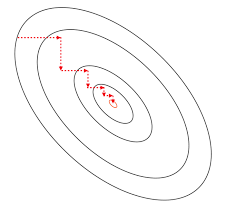
\includegraphics[width=0.9\linewidth]{coordinate_descent.png} 
\caption{Наглядное представление метода}
\label{fig:wrapfig}
\end{wrapfigure}

Рассмотрим один из наиболее простых методов многометрной оптимизации - \textbf{координатный спуск}. На каждой итерации происходит оптимизация по одной переменной, то есть происходит поиск минимума вдоль заданного направления.
Существуют различные порядки перебирания направлений поиска, в простейшем варианте они перебираются по порядку.\\

\begin{remark*}
Алгоритм не требует вычисления производной функции в точке.\\
\end{remark*}

\begin{algo*}
Пусть целевая функция имеет вид:
$f(x): \mathbb{X} \rightarrow \mathbb{R}$, где $\mathbb{X} \subset \mathbb{R}^n$

Задача оптимизации задана в следующем виде:
найти $x_{opt}:f(x_{opt}) = \min\limits_{x\in \mathbb{X}}f(x) = \mu$
\end{algo*}

\begin{itemize}
    \item Задать начальное приближение и точность расчёта: $X_0, \varepsilon$
    \item Рассчитать ${\displaystyle x_{i}^{k+1}={\underset {y\in \mathbb{X}_i }{\operatorname {arg\,min} }}\;f(x_{1}^{k+1},\dots ,x_{i-1}^{k+1},y,x_{i+1}^{k},\dots ,x_{n}^{k})}$
    \item Проверить условие остановки (на усмотрение):
    \begin{itemize}
        \item $|x^{j}-x^{j+1}|<\varepsilon$
        \item $|F(x^{j})-F(x^{j+1})|<\varepsilon$
        \item иначе перейти к пункту 2
    \end{itemize}
\end{itemize}

Таким образом, на каждой итерации будет выполнено
${\displaystyle F({x} ^{0})\geqslant F({x} ^{1})\geqslant F({x} ^{2})\geqslant \dots .}$\\

\textbf{Реализация}
\begin{lstlisting}[language=Python]
def FastSearch(func_index, D, p, e_d, e_f, method):  # F(function), D(set), p(start point), e(error)
    while True:
        p_0 = p
        for index in range(len(p)):
            p = method(func_index, index, D[index][0], D[index][1], p, e_d, e_f)
        if (norm(p_0, p) < e_d) & (Functions[func_index * 2](p_0) - Functions[func_index * 2](p) < e_f):
            break

    best_point = p
    best_value = Functions[func_index * 2](p)
    return best_point, best_value
\end{lstlisting}


\begin{remark*}
Чтобы найти ${\displaystyle x_{i}^{k+1}={\underset {y\in \mathbb {X}_i }{\operatorname {arg\,min} }}\;f(x_{1}^{k+1},\dots ,x_{i-1}^{k+1},y,x_{i+1}^{k},\dots ,x_{n}^{k})}$ будем использовать метод золотого сечения и алгоритм глобальной одномерной оптимизации.   
\end{remark*}


\newpage 
\section{Градиентный спуск}

\begin{wrapfigure}{r}{0.25\textwidth}
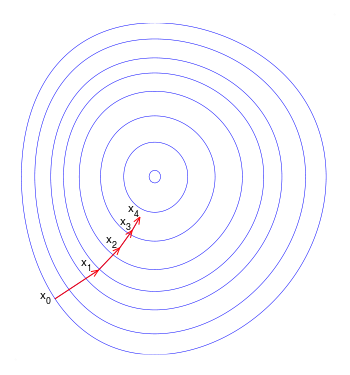
\includegraphics[width=0.9\linewidth]{gradient_descent.png} 
\caption{Наглядное представление метода}
\label{fig:wrapfig}
\end{wrapfigure}

Другой, не менее изветсный метод многомерной оптимизации - \textbf{градиентный спуск}. На каждой итерации вычисляется градиент функции в текущей точке, вдоль которого происходит поиск минимума вдоль направления.\\

\begin{remark*}
Алгоритм требует вычисления градиента функции в точке, поэтому необходимо, чтобы функция была дифференцируемой.\\
\end{remark*}

\begin{algo*}
Пусть целевая функция имеет вид:
$f(x): \mathbb{X} \rightarrow \mathbb{R}$, где $\mathbb{X} \subset \mathbb{R}^n$

Задача оптимизации задана в следующем виде:
найти $x_{opt}:f(x_{opt}) = \min\limits_{x\in \mathbb{X}}f(x) = \mu$


\begin{itemize}
    \item Задать начальное приближение и точность расчёта: $X_0, \varepsilon$
    \item Рассчитать $x^{j+1}=x^{j}-\lambda^{j} \nabla F\left(x^{j}\right)$
    \item Проверить условие остановки (на усмотрение):
    \begin{itemize}
        \item $|x^{j}-x^{j+1}|<\varepsilon$
        \item $|F(x^{j})-F(x^{j+1})|
        <\varepsilon$
        \item $\|\nabla F(x^{i})\|<\varepsilon$
        \item иначе перейти к пункту 2
    \end{itemize}
\end{itemize}

\end{algo*}

\begin{remark*}
$x^{j+1}=x^{j}-\lambda^{j} \nabla F\left(x^{j}\right)$, где $\lambda ^{j}$ задает скорость градиентного спуска и может быть выбрана как:
\begin{itemize}
    \item постоянная, тогда метод может не сходиться
    \item убывать по какому-то закону
    \item гарантировать наискорейший спуск\\
\end{itemize}
\end{remark*}


\textbf{Модификация: метод наискорейшего спуска}

В случае наискорейшего спуска $\lambda^{j}$ определяется как:
$$\lambda^{j}=\underset{\lambda}{\mathrm{argmin}} F\left(x^{j+1}\right) = \underset{\lambda}{\mathrm{argmin}}F\left(x^{j}-\lambda \nabla F\left(x^{j}\right)\right)$$

\begin{remark*}
Чтобы вычислить $\lambda^{j}$, будем использовать метод золотого сечения и алгоритм Moore-Skelboe.
\end{remark*}
\newpage 
\section{Метод золотого сечения}

\textbf{Метод золотого сечения} — это эффективный и простой способ нахождения локального минимума функции на заданном отрезке, за счет того, что на очередной итерации требует вычисления значения функции только в одной точке, что можеть быть очень важно, для сложновычислимых функций.

\begin{remark*}
Метод золотого сечения находит глобальный минимум только в случае унимодальных функций.
\end{remark*}

\begin{definition*}
Функция \textbf{унимодальная} на отрезке $[a, b]$, если $\exists \alpha, \beta: a\leq \alpha \leq \beta \leq b$ такие, что:

\begin{itemize}
    \item на отрезке $[a, \alpha]$ функция монотонно убывает
    \item на отрезке $[\beta, b]$ функция монотонно возрастает
    \item $\forall x \in [\alpha, \beta]: f(x) = \min\limits_{x\in[a,b]}f(x)$
\end{itemize}

\begin{figure}[h]
\centering
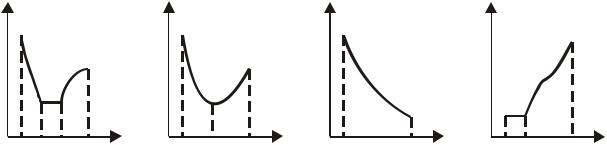
\includegraphics[scale=0.5]{unimodal_functions.jpg}
\caption{Примеры унимодальных функций}
\end{figure}
\end{definition*}

\textbf{Свойство.} Любой локальный минимум будет являться одновременно и глобальным минимумом.\\

\begin{wrapfigure}{l}{0.25\textwidth}
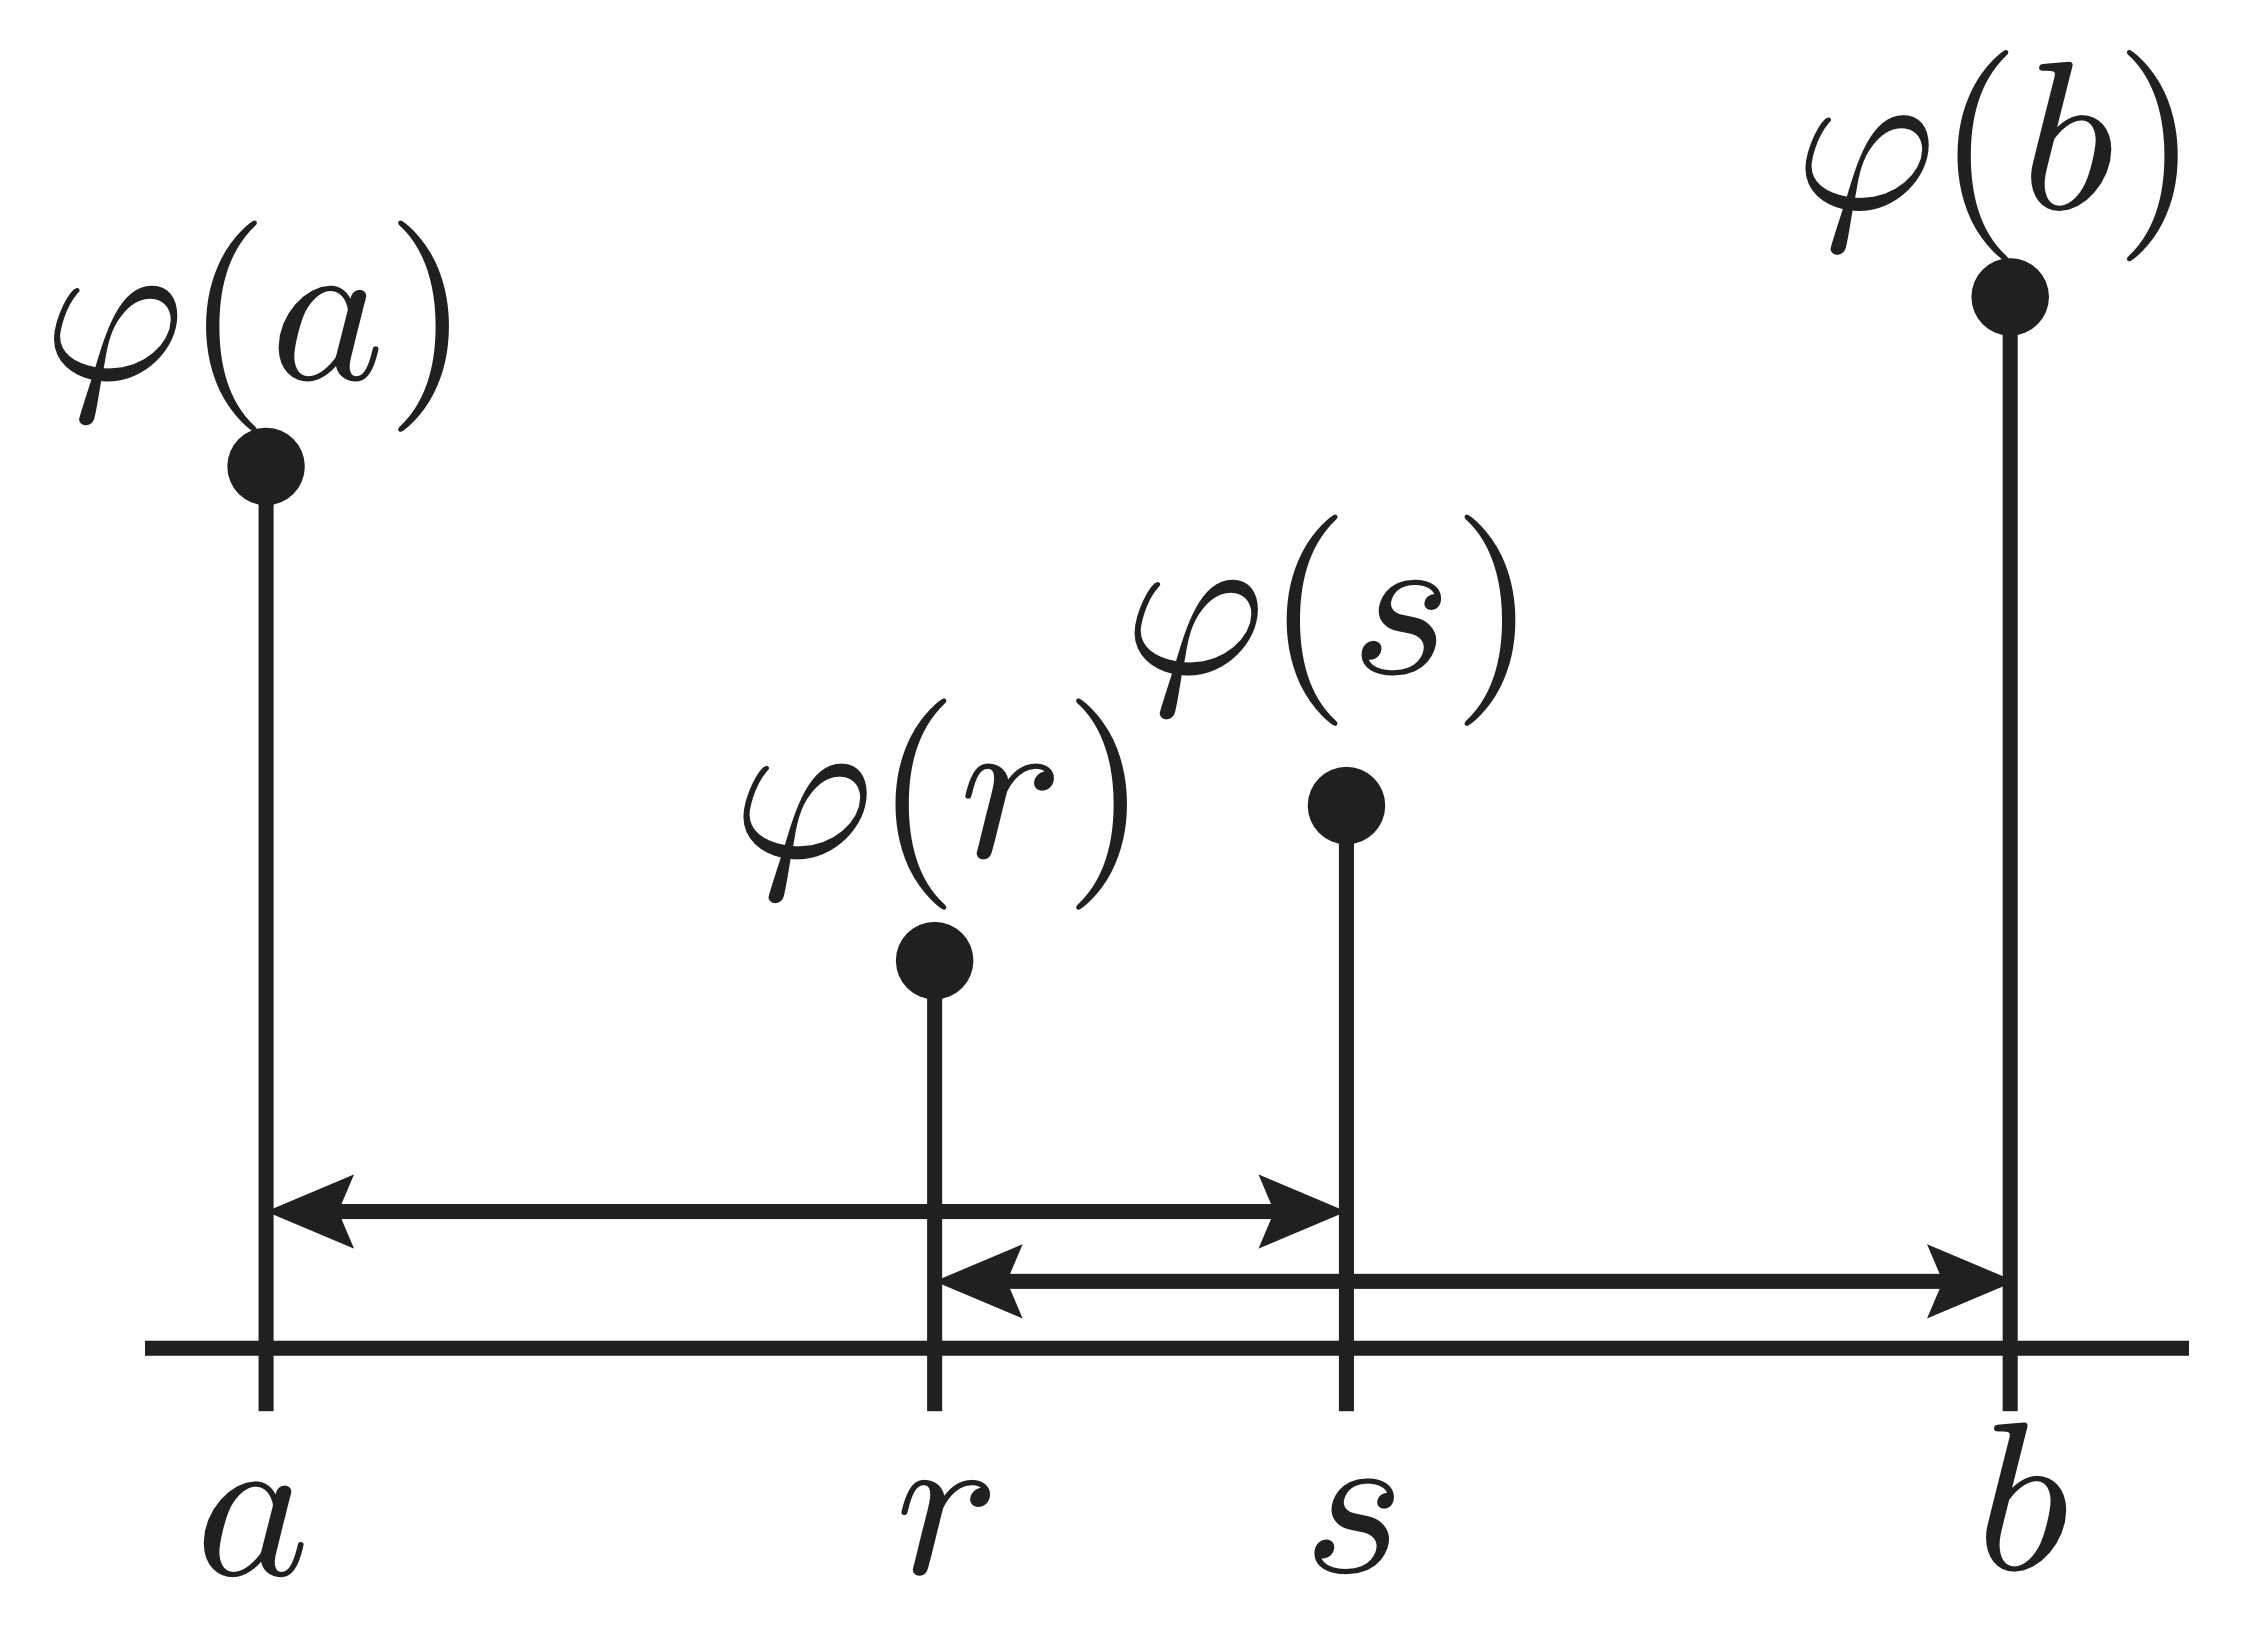
\includegraphics[width=0.9\linewidth]{golden_section.png} 
\caption{Итерация}
\label{fig:wrapfig}
\end{wrapfigure}

\textbf{Алгоритм.} Пусть хотим найти минимум функции $\varphi$ на отрезке $[a, b]$, разобъем его на три части двумя точками $r, s$ так, чтобы при отсекании одного из крайних подотрезков, одна из точек стала границей подотрезка для следующей итерации, то есть соотношение длин подотрезков оставалось прежним:\\

$|[a, r]|=|[s, b]|=l_1$

$|[r, s]|=l_2$

тогда, если $\varphi(r) \leq \varphi(s)$, то $s$ станет правой границей рассматриваемого отрезка, а $r$ станет правой внутренней точкой:\\

$$\frac{|[a, s]|}{|[a, b]|} = \frac{|[a, r]|}{|[a, s]|} \Rightarrow \frac{l_1+l_2}{2l_1+l_2} = \frac{l_1}{l_1+l_2} \Rightarrow l_1^2-l_1\cdot{l_2}-l_2^2=0 \Rightarrow \frac{l_1}{l_2}=\frac{1+\sqrt{5}}{2}=\Phi \approx 1.618$$\\

\begin{remark*}
Число $\Phi$ называют \textbf{золотым сечением}
\end{remark*}

Несмотря на то, что данный метод гарантированно находит глобальный минимум только для унимодальных функций, мы будем его использовать для сравнения с более надежными методами.

\textbf{Реализация}\\

\begin{lstlisting}[language=Python]
def GoldenRatio(func_index, index, a, b, p, e_d, e_f):  # f(function), i(index of direction),
    # a(left border), b(right border), p(current point), e_d(error of d), e_f(error of f)
    F = Functions[func_index * 2]
    phi = (1 + np.sqrt(5)) / 2  # constant of golden ratio
    x_1 = b - (b - a) / phi
    x_2 = a + (b - a) / phi
    p_1 = p.copy()  # current point
    p_2 = p.copy()  # current point
    p_1[index] = x_1
    p_2[index] = x_2
    f_1 = F(p_1)  # value in 1-st point
    f_2 = F(p_2)  # value in 2-nd point
    while (b - a > e_d) | (abs(f_1 - f_2) > e_f):  # termination criteria
        if f_1 <= f_2:
            b = x_2
            x_2 = x_1
            x_1 = b - (b - a) / phi

            p_1[index] = x_1
            p_2[index] = x_2

            f_2 = f_1
            f_1 = F(p_1)
        else:
            a = x_1
            x_1 = x_2
            x_2 = a + (b - a) / phi

            p_1[index] = x_1
            p_2[index] = x_2

            f_1 = f_2
            f_2 = F(p_2)

    best_point = []
    for i in range(len(p)):
        best_point.append((p_1[i] + p_2[i]) / 2)

    return best_point  # point of extremum with error e_d
\end{lstlisting}

\textbf{Сложность}\\

На каждой итерации длина рассматриваемого отрезка умножается на $$\frac{l_1+l_2}{l_1+l_2+l_2}=\frac{3+\sqrt{5}}{4+2\sqrt{5}}=\Phi^{-1} = \phi$$\\
Для достижения точности $\delta$ потребуется $$\frac{\ln(\frac{|[a, b]|}{\delta})}{\ln(\Phi)} \approx 2\ln(\frac{|[a, b]|}{\delta})$$ итераций.
\newpage 
\section{Глобальная одномерная оптимизация}
Алгоритм поиска глобального минимума функции вдоль одного направления будет основываться на интервальном анализе. Приведем основные определения и теоремы, которые нам пригодятся для посторения алгоритма.

\begin{definition*}
Интервалом $[a, b]$ называется следующее множество:
$$[a,b]:=\{x \in \mathbb{R} | a \le x \le b\}$$

в других обозначениях:
$$\bold{x}:=[\bold{\underline{x}},\bold{\overline{x}}]$$где $\bold{\underline{x}},\bold{\overline{x}}$ - левая и правая граница интервала соответственно.
\end{definition*}

\textbf{Арифметические свойства интервалов.}
\begin{itemize}

    \item $\bold{x} + \bold{y} = [{\bold{\underline{x}} + \bold{\underline{y}},  \bold{\overline{x}} + \bold{\overline{y}}}]$

    \item $\bold{x} - \bold{y} = [{\bold{\underline{x}} - \bold{\overline{y}},  \bold{\overline{x}} - \bold{\underline{y}}}]$

    \item $\bold{x} \cdot \bold{y} = [min(\bold{\underline{x} \underline{y}}, \bold{\underline{x} \overline{y}}, \bold{\overline{x} \underline{y}}, \bold{\overline{x} \overline{y}}) , max(\bold{\underline{x} \underline{y}}, \bold{\underline{x} \overline{y}}, \bold{\overline{x} \underline{y}}, \bold{\overline{x} \overline{y}})]$

    \item $\bold{x} / \bold{y} = \bold{x} \cdot[1/\bold{\overline{y}}, 1/\bold{\underline{y}}]$, если $\bold{\underline{y}} > 0$
\end{itemize}

\begin{example*}
Пусть известно, что первый гонщик проезжает длину гонки за время от 80 до 100 минут, а второй от 85 до 90 минут, какая может быть разница во времени приезда к финишу?

Воспользуемся вторым арифметическим свойством:

$\bold{T_1} = [80, 100]$

$\bold{T_2} = [85, 90]$, тогда результатом будет интервал $\bold{T_1} - \bold{T_2} = [80-90, 100-85] = [-10, 15]$

То есть первый гонщик может как приехать на 10 минут раньше, так и задержаться на 15 минут.
\end{example*}

\begin{remark*}
Так как интервалы являются множествами, то для них можно определить частичный порядок относительно включения:

$$\bold{a} \subseteq \bold{b} \iff \bold{\underline{b}} \leq \bold{\underline{a}} \cap \bold{\overline{a}} \leq \bold{\underline{b}}$$

\end{remark*}

\begin{property*}
Интервалы обладают свойством монотонности относительно арифметических операций:

Пусть $\bold{a} \subseteq \bold{a'}, \bold{b} \subseteq \bold{b'}, \star \subseteq \{+, -, \cdot, /\}$, тогда $\bold{a} \star \bold{b} \subseteq \bold{a'} \star \bold{b'}$
\end{property*}

\begin{theorem*}{Основная теорема интервальной арифметики}\\
Пусть $f(x_1, ..., x_n)$ - функция вещественных аргументов $x_1, ..., x_n$, и для нее определен результат $\bold{F(X_1, ..., X_n)}$ подстановки вместо аргументов интервалов которые они пробегают $\bold{(X_1, ..., X_n)} \subset \mathbb{IR}^n$ и для $\bold{(X_1, ..., X_n)}$ операциии выполняются по правилам интервальной арифметики. Тогда выполнено следущее:
    \begin{gather*}
        \{f(x_1,...,x_n) | x_1 \in \bold{X_1},...,x_n \in \bold{X_n}\} \subseteq \bold{F(\bold{X_1},...,\bold{X_n}})
    \end{gather*}
\end{theorem*}


\begin{proposition*}
Пусть $f(x_1, ..., x_n)$ - функция вещественных аргументов $x_1, ..., x_n$, и $\bold{F(X_1, ..., X_n)}$ соответствующая ей интервальная функция, тогда выполняется монотонность по включению:\\
Пусть $\bold{X_1},...,\bold{X_n}$ и $\bold{Y_1},...,\bold{Y_n}$, такие что $\bold{X_1} \subseteq \bold{Y_1},...,\bold{X_n} \subseteq \bold{Y_n}$, тогда:
$$\bold{F(X_1, ..., X_n)} \subseteq \bold{F(Y_1, ..., Y_n)}$$
\end{proposition*}

\begin{definition*}
Пусть $N > 0$  натуральное число, тогда если $\langle S_0,..., S_{n-1} \rangle$ семейство непустых подмножеств множества $S$, тогда будем называть его покрытием внутри $S$. В частности, если обьединение $S_0,..., S_{n-1}$ равно $S$, тогда последовательность $\langle S_0,..., S_{n-1} \rangle$ является покрытием $S$.
\end{definition*}


\begin{theorem*}
Рассмотрим задачу глобальной оптимизации. Пусть $\langle B_0,..., B_{n-1} \rangle$ семейство множеств, содержащее глобальный минимум, такое что упорядочено по возрастанию нижней границы $\bold{F}(B_i)$ для $i=0, 1, 2,..., N-1$. Пусть $U$ наименьшее из верхних значений функции для подмножеств $\langle \bold{F}(B_0),..., \bold{F}(B_{n-1}) \rangle$. Тогда интервал $[lb(\bold{F}(B_0)), U]$ содержит глобальным минимум $\mu$.
\end{theorem*}

Используя данную теорию, напишем алгоритм поиска глобального минимума вдоль направления.

\subsection*{Алгоритм Moore-Skelboe}

\textbf{Реализация}\\

\begin{lstlisting}[language=Python]
def MooreSkelboe(func_index, index, a, b, p, e_d,
                 e_f):  # func_index(number of function in list of functions), index(index of direction),
    # a(left border), b(right border), p(current point), e_d(error of d), e_f(error of f)
    F = Functions[func_index * 2 + 1]
    interval_d = []
    for i in range(len(p)):
        interval_d.append(interval[p[i], p[i]])
    interval_d[index] = interval[a, b]

    interval_f = F(interval_d)
    set_of_intervals = [[interval_d, interval_f]]
    U = right(interval_f)
    w_f = right(interval_f) - left(interval_f)
    w_d = right(interval_d[index]) - left(interval_d[index])
    best_interval = set_of_intervals[0]
    while (w_d > e_d) | (w_f > e_f):
        set_of_intervals.pop(0)
        mid_p = mid(best_interval[0][index])
        interval_1 = best_interval[0].copy()
        interval_2 = best_interval[0].copy()
        interval_1[index] = interval[left(best_interval[0][index]), mid_p]
        interval_1_f = F(interval_1)
        interval_2[index] = interval[mid_p, right(best_interval[0][index])]
        interval_2_f = F(interval_2)
        U = min(U, right(interval_1_f))
        U = min(U, right(interval_2_f))

        for i in range(len(set_of_intervals)):
            if U < left(set_of_intervals[i][1]):
                set_of_intervals = set_of_intervals[:i]
                break

        val_1 = left(interval_1_f)
        val_2 = left(interval_2_f)

        if (len(set_of_intervals) == 0) or (val_1 > left(
                set_of_intervals[-1][1])):
            set_of_intervals.append([interval_1, interval_1_f])
        else:
            l = 0
            r = len(set_of_intervals) - 1
            while l < r:
                m = int((l + r) / 2)
                if left(set_of_intervals[m][1]) > val_1:
                    r = m
                else:
                    l = m + 1
            set_of_intervals.insert(l, [interval_1, interval_1_f])

        if val_2 > left(set_of_intervals[-1][1]):
            set_of_intervals.append([interval_2, interval_2_f])
        else:
            l = 0
            r = len(set_of_intervals) - 1
            while l < r:
                m = int((l + r) / 2)
                if left(set_of_intervals[m][1]) > val_2:
                    r = m
                else:
                    l = m + 1
            set_of_intervals.insert(l, [interval_2, interval_2_f])

        best_interval = set_of_intervals[0]
        w_f = right(best_interval[1]) - left(best_interval[1])
        w_d = right(best_interval[0][index]) - left(best_interval[0][index])

    best_point = []
    for i in range(len(p)):
        best_point.append(mid(best_interval[0][i]))

    return best_point
\end{lstlisting}


\textbf{Сложность}\\

На каждой итерации длина одного из интервалов в семейсмве интервалов делится на 2. Каждая итерация совершается за O(log(size)).
Для достижения точности $\delta$ потребуется $$\frac{\ln(\frac{|[a, b]|}{\delta})}{\ln(\Phi)} \approx 2\ln(\frac{|[a, b]|}{\delta})$$ итераций.
\newpage 
\section{Тестирование}
    Ниже приведены результаты тестирования двух методов оптимизации на тестовых функциях, первый использует метод золотого сечения, для поиска минимума вдоль направления, а другой алгоритм Moore-Skelboe.

    \subsection*{Функция Растригина}

    \subsubsection*{График функции при $n=2$}
    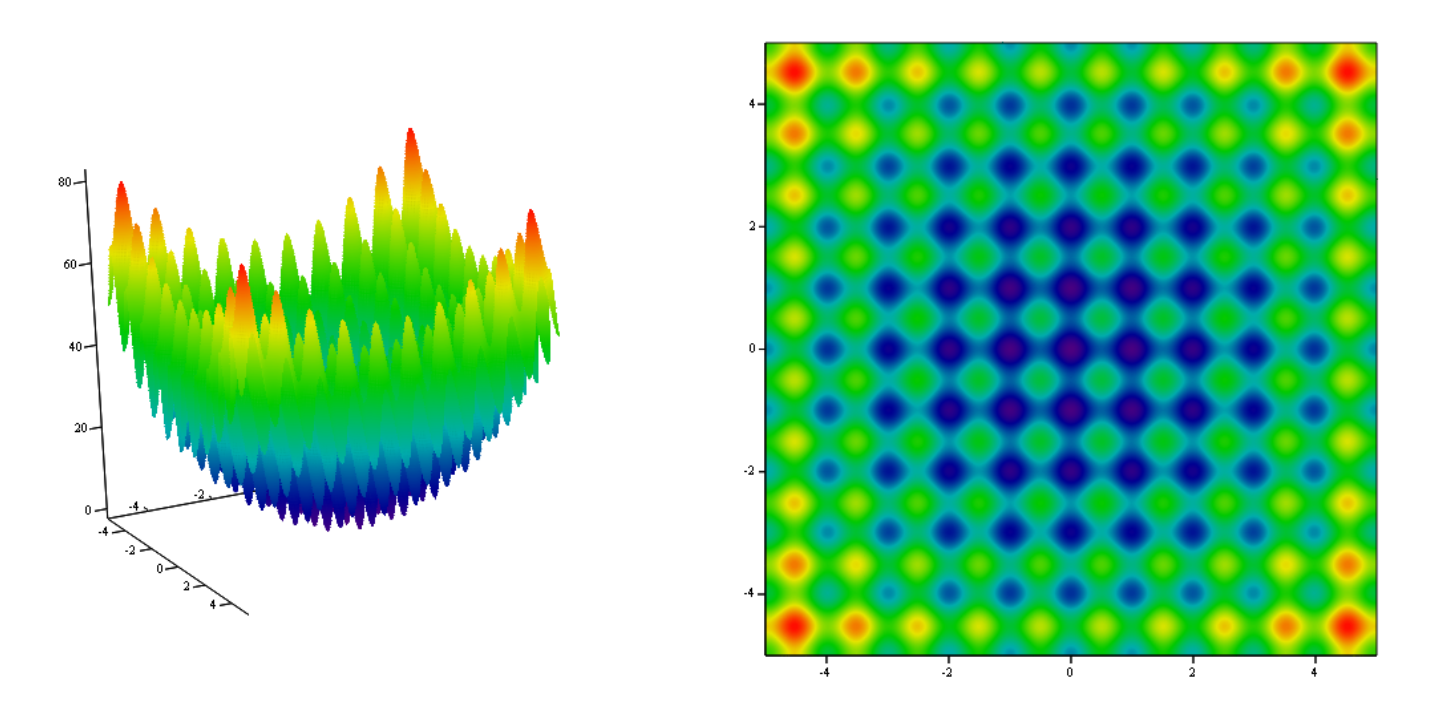
\includegraphics[width=16cm, height=8cm]{Rastrigin}

    \subsubsection*{Формула}
    \begin{gather*}
        f(x)=10 n+\sum_{i=1}^n\left(x_i^2-10 \cdot \cos \left(2 \pi \cdot x_i\right)\right)
    \end{gather*}

    \subsubsection*{Результаты тестирования}

    \begin{tabular}{ |p{2cm}|p{2cm}|p{3cm}|p{2cm}|p{4cm}|  }
        \hline
        n  & точность & метод         & время   & минимум                \\
        \hline
        5  & $10^-3$  & Golden ratio  & 2.22 ms & 4.974821275706137      \\\cline{2-5}
        & $10^-3$  & Moore-Skelboe & 178 ms  & 9.238348694395881e-05  \\
        \hline
        10 & $10^-3$  & Golden ratio  & 4.78 ms & 9.94964255141227       \\\cline{2-5}
        & $10^-3$  & Moore-Skelboe & 736 ms  & 0.00018476697390212848 \\
        \hline
        20 & $10^-3$  & Golden ratio  & 13.3 ms & 19.899285102824635     \\\cline{2-5}
        & $10^-3$  & Moore-Skelboe & 2.52 s  & 0.0003695339478184678  \\
        \hline
        30 & $10^-3$  & Golden ratio  & 24.1 ms & 29.84892765423696      \\\cline{2-5}
        & $10^-3$  & Moore-Skelboe & 5.38 s  & 0.0005543009217348072  \\
        \hline
        40 & $10^-3$  & Golden ratio  & 43.2 ms & 39.79857020564907      \\\cline{2-5}
        & $10^-3$  & Moore-Skelboe & 9.58 s  & 0.0007390678956511465  \\
        \hline
        50 & $10^-3$  & Golden ratio  & 58.8 ms & 49.748212757061154     \\\cline{2-5}
        & $10^-3$  & Moore-Skelboe & 14.9 s  & 0.0009238348695674858  \\
        \hline

    \end{tabular}

    \subsection*{Функция Растригина новгородская}

    \subsubsection*{График функции при $n=2$}
    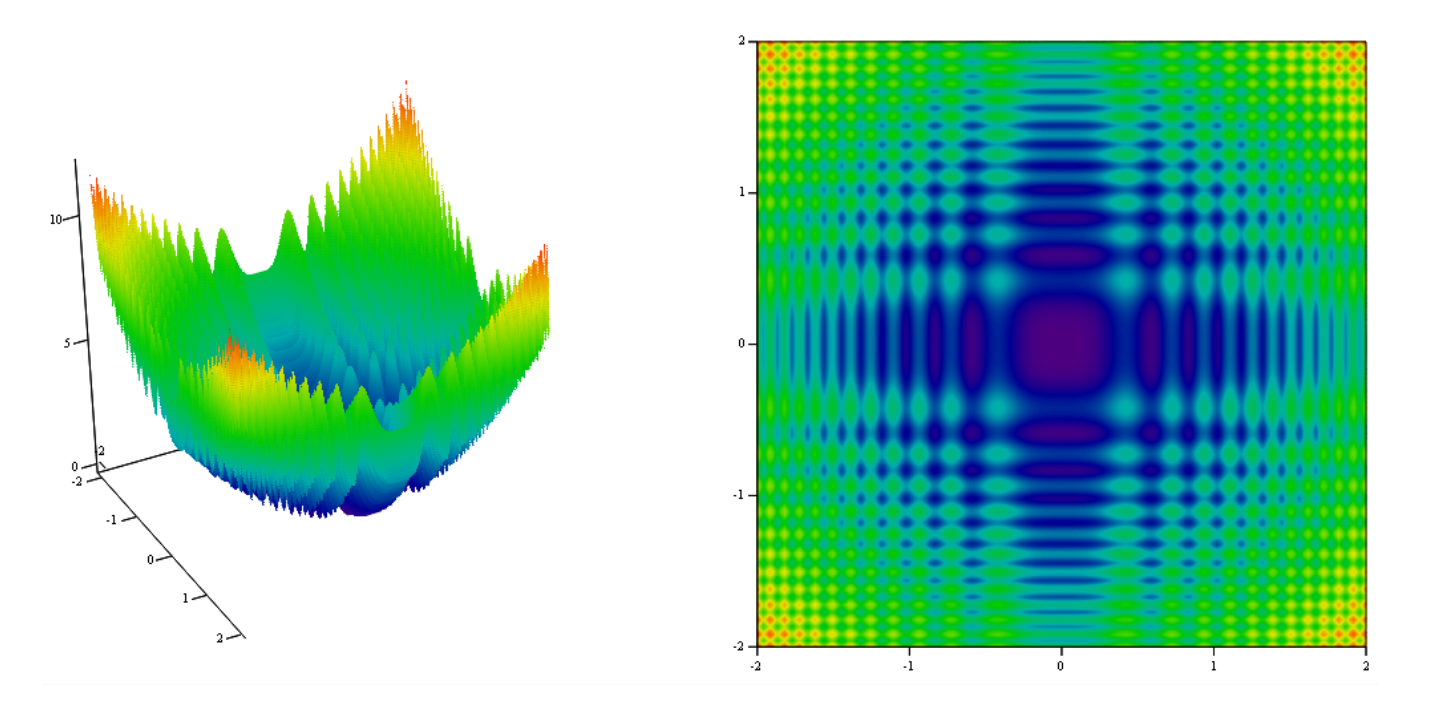
\includegraphics[width=16cm, height=8cm]{Rastrigin_new}

    \subsubsection*{Формула}
    \begin{gather*}
        f(x)=n+\sum_{i=1}^n\left(x_i^2-\cos \left(18 \cdot x_i^2\right)\right)
    \end{gather*}

    \subsubsection*{Результаты тестирования}

    \begin{tabular}{ |p{2cm}|p{2cm}|p{3cm}|p{2cm}|p{4cm}|  }
        \hline
        n  & точность & метод         & время   & значение              \\
        \hline
        5  & $10^-3$  & Golden ratio  & 1.36 ms & 1.542458003137213     \\\cline{2-5}
        & $10^-3$  & Moore-Skelboe & 151 ms  & 0.0007449817996270092 \\
        \hline
        10 & $10^-3$  & Golden ratio  & 5.18 ms & 3.0849160062744287    \\\cline{2-5}
        & $10^-3$  & Moore-Skelboe & 636 ms  & 0.0014899635992544624 \\
        \hline
        20 & $10^-3$  & Golden ratio  & 20.8 ms & 6.16983201254885      \\\cline{2-5}
        & $10^-3$  & Moore-Skelboe & 1.94 s  & 0.002979927198509369  \\
        \hline
        30 & $10^-3$  & Golden ratio  & 37 ms   & 9.254748018823253     \\\cline{2-5}
        & $10^-3$  & Moore-Skelboe & 4.54 s  & 0.0044698907977642754 \\
        \hline
        40 & $10^-3$  & Golden ratio  & 54.2 ms & 12.339664025097658    \\\cline{2-5}
        & $10^-3$  & Moore-Skelboe & 7.79 s  & 0.005959854397019182  \\
        \hline
        50 & $10^-3$  & Golden ratio  & 79.7 ms & 15.424580031372061    \\\cline{2-5}
        & $10^-3$  & Moore-Skelboe & 11.6 s  & 0.0074498179962740885 \\
        \hline

    \end{tabular}

    \subsection*{Функция Розенброка}

    \subsubsection*{График функции при $n=2$}
    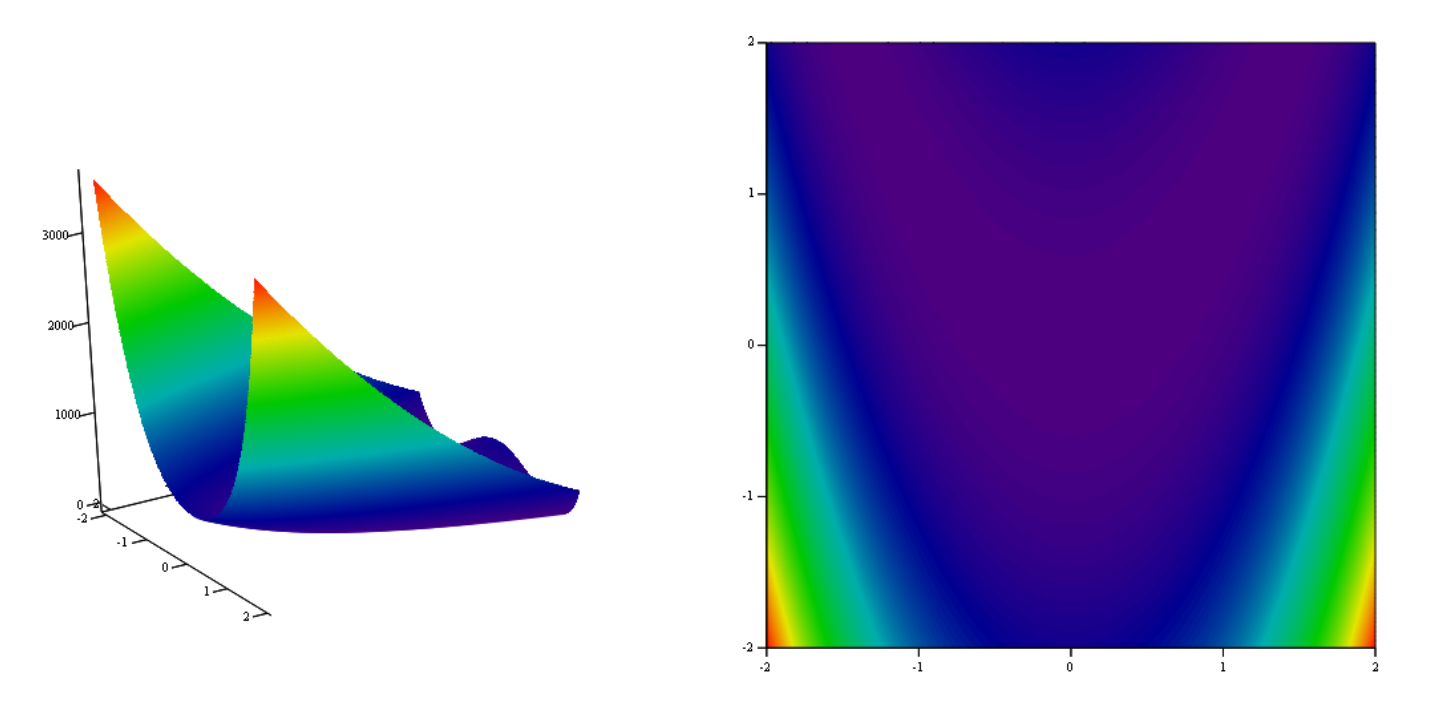
\includegraphics[width=16cm, height=8cm]{Rozenbrock}

    \subsubsection*{Формула}
    \begin{gather*}
        f(x)=\sum_{i=1}^{n-1}\left(100\left(x_{i+1}-x_i^2\right)^2+\left(1-x_i\right)^2\right)
    \end{gather*}

    \subsubsection*{Результаты тестирования}

    \begin{tabular}{ |p{2cm}|p{2cm}|p{3cm}|p{2cm}|p{4cm}|  }
        \hline
        n & точность & метод         & время   & значение            \\
        \hline
        2 & $10^-3$  & Golden ratio  & 1.12 ms & 0.16956582889643249 \\\cline{2-5}
        & $10^-3$  & Moore-Skelboe & 155 ms  & 0.16036252999621464 \\
        \hline
        3 & $10^-3$  & Golden ratio  & 5.95 ms & 0.259397310396006   \\\cline{2-5}
        & $10^-3$  & Moore-Skelboe & 3.99 s  & 0.11254106932659813 \\
        \hline
        4 & $10^-3$  & Golden ratio  & 17 ms   & 0.28064340055794645 \\\cline{2-5}
        & $10^-3$  & Moore-Skelboe & 8.75 s  & 0.11734786681147619 \\
        \hline
        5 & $10^-3$  & Golden ratio  & 27.3 ms & 0.2830939134564683  \\\cline{2-5}
        & $10^-3$  & Moore-Skelboe & 15.6 s  & 0.11851270446807871 \\
        \hline
        6 & $10^-3$  & Golden ratio  & 40.4 ms & 0.29047947563212634 \\\cline{2-5}
        & $10^-3$  & Moore-Skelboe & 24.5 s  & 0.11879389607067276 \\
        \hline
        7 & $10^-3$  & Golden ratio  & 49.2 ms & 0.29064024190256904 \\\cline{2-5}
        & $10^-3$  & Moore-Skelboe & 35.6 s  & 0.1136410373197746  \\
        \hline
        8 & $10^-3$  & Golden ratio  & 18.5 ms & 0.33244082803407593 \\\cline{2-5}
        & $10^-3$  & Moore-Skelboe & 41.7 s  & 0.14015453688727936 \\
        \hline

    \end{tabular}

    \subsection*{Функция Экли}

    \subsubsection*{График функции при $n=2$}
    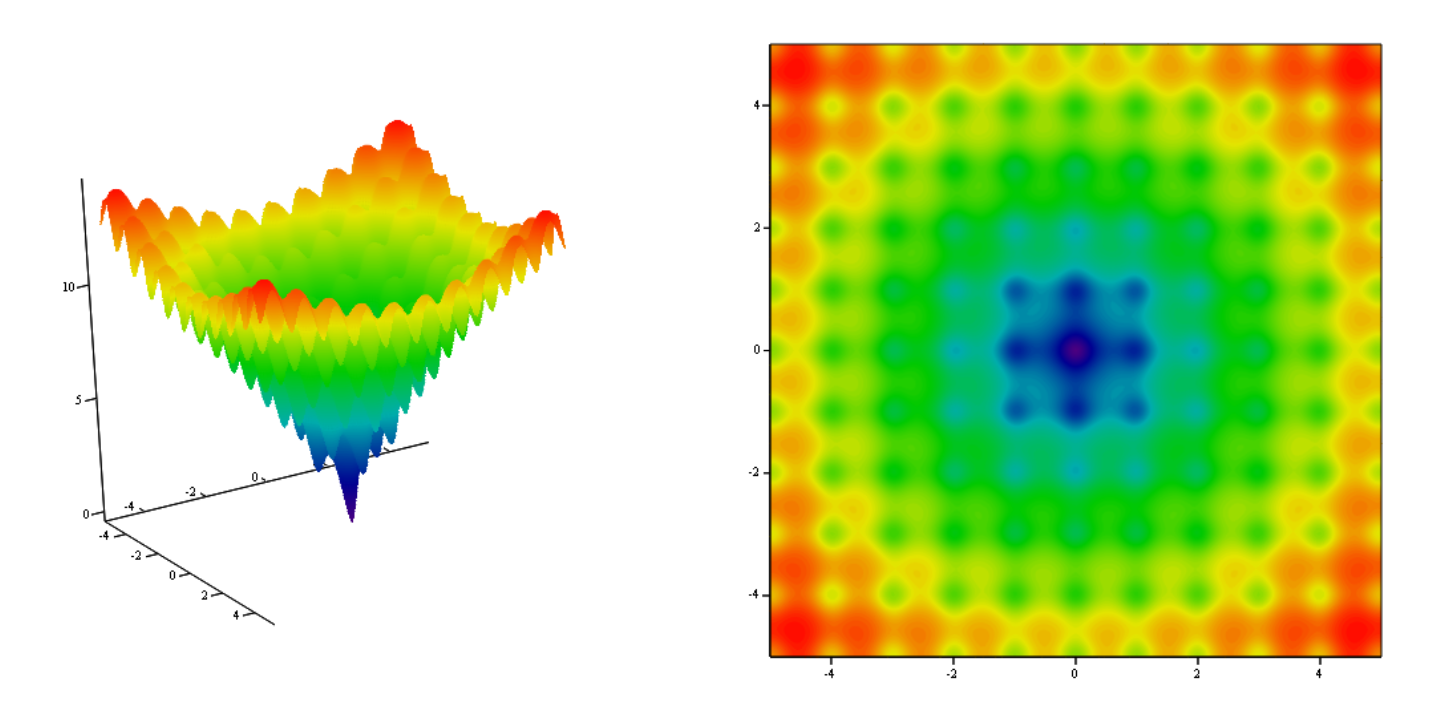
\includegraphics[width=16cm, height=8cm]{Ackley}

    \subsubsection*{Формула}
    \begin{gather*}
        f(x)=20+e-20 e^{-0.2 \sqrt{\frac{1}{n} \sum_{i=1}^n x_i^2}}-e^{\frac{1}{n} \sum_{i=1}^n \cos \left(2 \pi \cdot x_i\right)}
    \end{gather*}

    \subsubsection*{Результаты тестирования}

    \begin{tabular}{ |p{2cm}|p{2cm}|p{3cm}|p{2cm}|p{4cm}|  }
        \hline
        n  & точность & метод         & время   & значение               \\
        \hline
        5  & $10^-3$  & Golden ratio  & 2.41 ms & -4.440892098500626e-16 \\\cline{2-5}
        & $10^-3$  & Moore-Skelboe & 553 ms  & 0.0012256630393632229  \\
        \hline
        20 & $10^-3$  & Golden ratio  & 9.06 ms & 3.5744545080266543     \\\cline{2-5}
        & $10^-3$  & Moore-Skelboe & 1.35 s  & 0.0012256630393632229  \\
        \hline
        20 & $10^-3$  & Golden ratio  & 30.6 ms & 3.5744545080266543     \\\cline{2-5}
        & $10^-3$  & Moore-Skelboe & 3.41 s  & 0.0012256630393632229  \\
        \hline
        30 & $10^-3$  & Golden ratio  & 58.5 ms & 3.574454508026655      \\\cline{2-5}
        & $10^-3$  & Moore-Skelboe & 6.23 s  & 0.0012256630393645551  \\
        \hline
        40 & $10^-3$  & Golden ratio  & 84.1 ms & 3.574454508026654      \\\cline{2-5}
        & $10^-3$  & Moore-Skelboe & 10.6 s  & 0.0012256630393632229  \\
        \hline
        50 & $10^-3$  & Golden ratio  & 124 ms  & 3.5744545080266525     \\\cline{2-5}
        & $10^-3$  & Moore-Skelboe & 14.9 s  & 0.0012256630393618906  \\
        \hline

    \end{tabular}

    \subsection*{Функция Гриванка}

    \subsubsection*{График функции при $n=2$}
    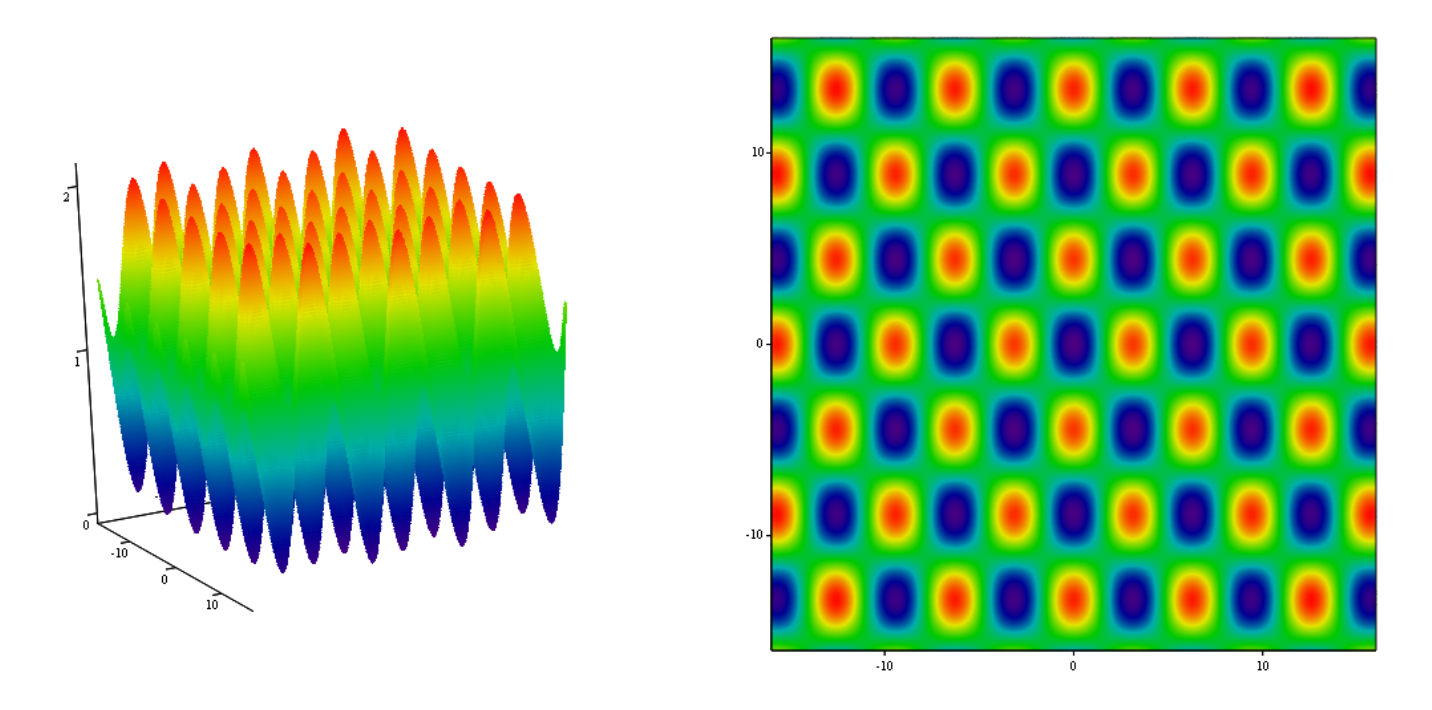
\includegraphics[width=16cm, height=8cm]{Grivank}

    \subsubsection*{Формула}
    \begin{gather*}
        f(x)=\sum_{i=1}^n \frac{x_i^2}{4000}-\prod_{i=1}^n \cos \left(\frac{x_i}{\sqrt{i}}\right)+1
    \end{gather*}

    \subsubsection*{Результаты тестирования}

    \begin{tabular}{ |p{2cm}|p{2cm}|p{3cm}|p{2cm}|p{4cm}|  }
        \hline
        n  & точность & метод         & время   & значение               \\
        \hline
        5  & $10^-3$  & Golden ratio  & 2.41 ms & 0.009864698515380743   \\\cline{2-5}
        & $10^-3$  & Moore-Skelboe & 183 ms  & 1.0644240466817223e-07 \\
        \hline
        10 & $10^-3$  & Golden ratio  & 6.05 ms & 0.009864698515380743   \\\cline{2-5}
        & $10^-3$  & Moore-Skelboe & 739 ms  & 1.3662353537391425e-07 \\
        \hline
        20 & $10^-3$  & Golden ratio  & 21.4 ms & 0.009864698515380743   \\\cline{2-5}
        & $10^-3$  & Moore-Skelboe & 2.44 s  & 1.6799845647952338e-07 \\
        \hline
        30 & $10^-3$  & Golden ratio  & 40.2 ms & 0.009864698515380743   \\\cline{2-5}
        & $10^-3$  & Moore-Skelboe & 5.16 s  & 1.867295605917363e-07  \\
        \hline
        40 & $10^-3$  & Golden ratio  & 59.3 ms & 0.009864698515380743   \\\cline{2-5}
        & $10^-3$  & Moore-Skelboe & 9.09 s  & 2.0016648982768004e-07 \\
        \hline
        50 & $10^-3$  & Golden ratio  & 84.4 ms & 0.009864698515380743   \\\cline{2-5}
        & $10^-3$  & Moore-Skelboe & 14 s    & 2.1067470723501458e-07 \\
        \hline

    \end{tabular}

    \subsection*{Функция Швефеля}

    \subsubsection*{График функции при $n=2$}
    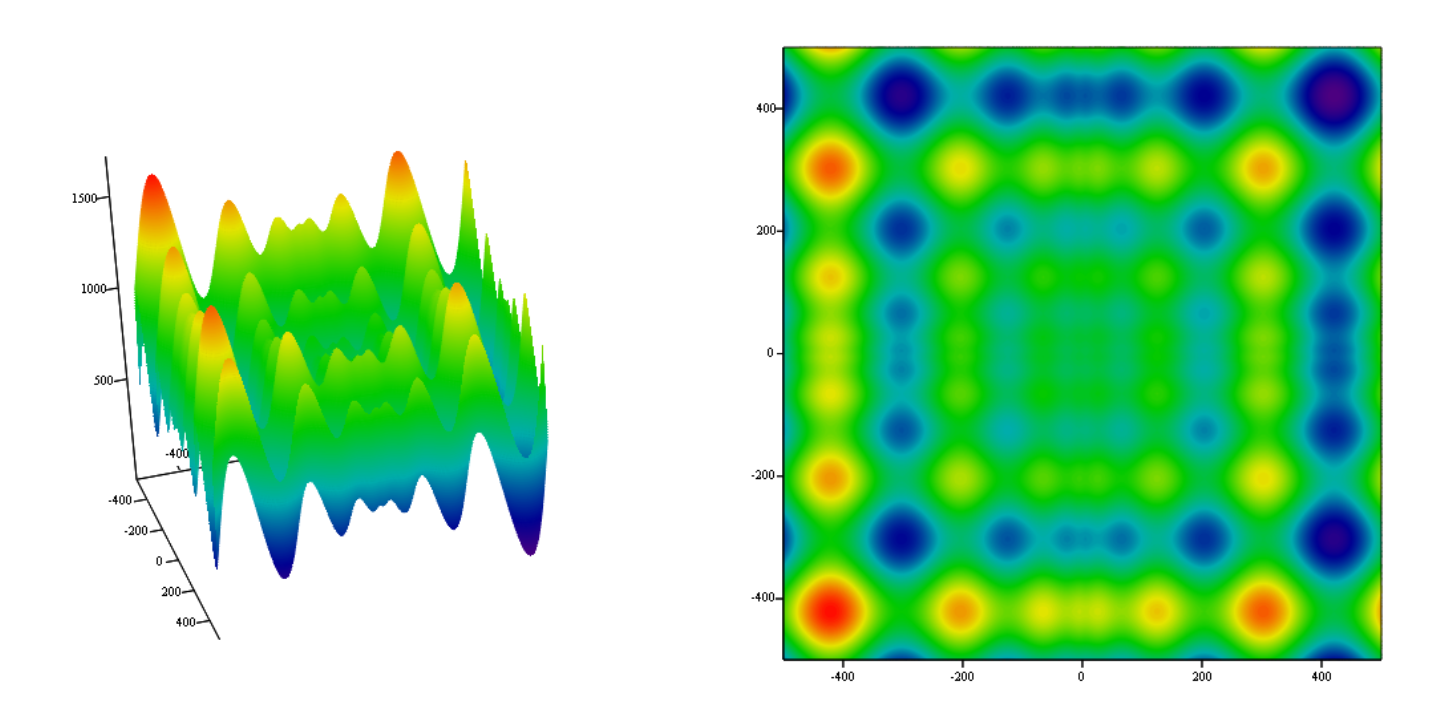
\includegraphics[width=16cm, height=8cm]{Shvefel}

    \subsubsection*{Формула}
    \begin{gather*}
        f(x)=418.9829 n-\sum_{i=1}^n\left(x_i \sin \left(\sqrt{\left|x_i\right|}\right)\right)
    \end{gather*}

    \subsubsection*{Результаты тестирования}

    \begin{tabular}{ |p{2cm}|p{2cm}|p{3cm}|p{2cm}|p{4cm}|  }
        \hline
        n & точность & метод         & время   & значение               \\
        \hline
        2 & $10^-3$  & Golden ratio  & 721 µs  & 236.8766946858181      \\\cline{2-5}
        & $10^-3$  & Moore-Skelboe & 4.98 s  & 2.5455285594944144e-05 \\
        \hline
        3 & $10^-3$  & Golden ratio  & 800 µs  & 355.3150420287272      \\\cline{2-5}
        & $10^-3$  & Moore-Skelboe & 9.41 s  & 3.8182928392416216e-05 \\
        \hline
        4 & $10^-3$  & Golden ratio  & 1.44 ms & 473.7533893716363      \\\cline{2-5}
        & $10^-3$  & Moore-Skelboe & 15 s    & 5.091057118988829e-05  \\
        \hline
        5 & $10^-3$  & Golden ratio  & 1.4 ms  & 592.1917367145454      \\\cline{2-5}
        & $10^-3$  & Moore-Skelboe & 22 s    & 6.363821398736036e-05  \\
        \hline
        6 & $10^-3$  & Golden ratio  & 2.19 ms & 710.6300840574543      \\\cline{2-5}
        & $10^-3$  & Moore-Skelboe & 31.1 s  & 7.636585655745876e-05  \\
        \hline
        7 & $10^-3$  & Golden ratio  & 1.88 ms & 829.0684314003631      \\\cline{2-5}
        & $10^-3$  & Moore-Skelboe & 40 s    & 8.909349912755715e-05  \\
        \hline
        8 & $10^-3$  & Golden ratio  & 4.92 ms & 947.5067787432718      \\\cline{2-5}
        & $10^-3$  & Moore-Skelboe & 52 s    & 0.00010182114169765555 \\
        \hline

    \end{tabular}

\newpage





\section{Примеры} 
\subsection{Ссылки на статьи}

Ссылки на статьи оформляются с помощью пакета \texttt{biblatex}, например~\cite{chirkova18}. В описании статье в bib файле нужно обязательно указывать место публикации работы (журнал или конференцию) и год. Обратите внимание, что для описания статей из разных источников в списке литературы используются разные команды в bib файле: статья из журнала~\cite{ctan}, статья с конференции~\cite{chirkova18}, книга~\cite{knuth-acp}, глава книги~\cite{knuth-fa}. Если статься еще не опубликована нигде, а только выложена на arXiv, то на нее тоже можно сослаться~\cite{chirkova18_arxiv}, но предпочтительно ссылаться на опубликованную версию, если она уже существует. Если вы хотите сослаться на сайт, то можно либо так же внести его в список литературы~\cite{knuthwebsite} (рекомендуется, если таких ссылок у вас много из-за особенностей темы вашего проекта), либо использовать ссылку внизу страницы\footnote{Книги доступны по ссылке: \url{http://www-cs-faculty.stanford.edu/~uno/abcde.html}, дата обр. 16.05.2013}. При работе с онлайн ресурсами не забывайте указывать дату обращения к этому ресурсу, так как в отличие от опубликованных статей, эти ресурсы могут измениться в любой момент.

\subsection{Рисунки}

\begin{figure}[ht]
	\centering
	\includegraphics[width=0.8\textwidth]{example.png}
	\caption{Пример графика. Тут должна быть подпись, поясняющая что происходит на рисунке (краткая, но достаточная для понимания основной идеи графика).}
	\label{fig:by_epochs}
\end{figure}

Все рисунки в тексте должны иметь подписи и вы на них должны ссылаться в тексте. Например, на Рисунке~\ref{fig:by_epochs} изображен пример графика. Не забывайте подписывать все оси на графиках, добавлять легенду и пояснять все обозначения, а также используйте адекватного размера шрифты и толщину линий на графиках (все должно быть видно и понятно без многократного увеличения). На рисунке из примера явно не хватает обозначения синей линии в легенде.


\subsection{Таблицы}

Все таблицы в тексте тоже должны иметь подписи и вы на них должны ссылаться в тексте. Например, в Таблице~\ref{table:long_epochs} показаны результаты примерного эксперимента. 


\begin{table}[ht]
	\caption{Пример таблички. Тут должна быть подпись, поясняющая что происходит в таблице (краткая, но по делу).}
	\label{table:long_epochs}
	\footnotesize
	\centering
	\begin{tabular}{lrrrrrrrr}
		\toprule
		& \multicolumn{3}{c}{$\mathsf{Val}$} &
		\multicolumn{3}{c}{$\mathsf{Test}$} \\
		\cmidrule(lr){2-4} \cmidrule(l){5-7} 
		{} &  $\mathsf{Prec}$ &  $\mathsf{Rec}$ &  $\mathsf{F1}$ &  $\mathsf{Prec}$ &  $\mathsf{Rec}$ &  $\mathsf{F1}$  &  $\mathsf{nodes}$ & $\mathsf{subtokens}$\\
		\midrule
		запуск 1    &    0.4894 &   0.3775 &  0.4263 &     0.4824 &    0.3683 &   0.4177 & 10029 & 179\\
		запуск 2    &    0.4887 &   0.3739 &  0.4237 &     0.4891 &    0.3724 &   0.4228 & 10039 & 177\\
		запуск 3    &    0.4820 &   0.3751 &  0.4219 &     0.4838 &    0.3677 &   0.4178 & 10037&	180\\
		\midrule
		\bf{среднее} &    \bf{0.4867} &   \bf{0.3755} &  \bf{0.4239} &    \bf{ 0.4851} &    \bf{0.3695} &   \bf{0.4195} \\
		\bf{дисперсия}  &    0.0041 &   0.0019 &  0.0022 &     0.0036 &    0.0025 &   0.0029 \\
		\bottomrule
	\end{tabular}
\end{table}

\subsection{Формулы}

Формулы стоит центрировать, а также нумеровать, если вы ссылаете на них в тексте. Также не забывайте пояснять все обозначения в формулах. Например, запишем следующую задачу оптимизации:
\begin{equation}
    \label{eq:si_opt}
        \theta* = \min_{\theta} F(\theta),
\end{equation}
где $F$~-- квадратичная функция от параметра $\theta$. При необходимости, далее в тексте можно сослаться на формулу~(\ref{eq:si_opt}). При этом, в зависимости от конкретных формул, можно использовать разные слова: формула, уравнение, задача оптимизации и т.п.


	
\newpage 
\printbibliography[heading=bibintoc] 

% \begin{thebibliography}{0}
% 	\bibitem{chirkova18}\hypertarget{chirkova18}{}
% 	\href{https://arxiv.org/abs/1810.10927}
% 	{Nadezhda Chirkova, Ekaterina Lobacheva, Dmitry Vetrov. Bayesian Compression for Natural Language Processing. In EMNLP 2018.}
% \end{thebibliography}
	
	
\end{document}
